\chapter{Grant Mitt: Concentration Before Diversification}

The episode opens with three claims before the formal interview even settles in: Grant Mitt did not diversify until the solar company had crossed a real revenue threshold; he would rather take risks early than arrive at wealth too late to use it; and he believes the operating skill, once learned, can be carried into a new circumstance. The mathematical content here is not physics, but the interview has a clear quantitative spine. It is a lesson in base rates, concentration, distribution, repeatable skill, scale, energy, and hiring under pressure.

\section{The Market Does Not Care How Old You Are}

The first formal question is about confidence. Mitt is young, the interviewer says, and he is operating in an industry where many owners may be two or three times his age. The answer comes in two pieces. First, if we make age a big deal, other people will make it a big deal. Second, once we are in the arena, business behaves more like a competitive selection mechanism than a credentialing committee.

Mitt reaches for the NFL analogy. A rookie can get cut. A nineteen-year veteran can get cut. A rookie can win, and a veteran can win. The analogy is not meant to erase experience; it is meant to put experience under the discipline of performance. The market does not choose a seller because the seller is older. It chooses according to the transaction.

A compact way to write the market test is
\begin{equation}
\text{customer choice}
=
f(\text{trust},\text{offer},\text{execution},\text{price},\text{timing}).
\end{equation}
Age can enter the transaction only if it changes one of those variables, especially trust. In Mitt's telling, the young founder's mistake is to let age become a reason before the market has even rendered judgment.

\begin{remark}
This equation is a reconstruction of the interview's logic, not a formula stated by Mitt. It records the order of explanation: the market chooses, and the operator's insecurity is not automatically one of the market's variables.
\end{remark}

That is the first pivot. Once age is put in its place, the interview can ask the harder question: if the market is so unforgiving, why start a business at all?

\section{The Bad Base Rates Of Starting}

Mitt's answer to the entrepreneurship question does not begin with romance. It begins with base rates. He warns that many people should be cautious about starting a business, and he supports that warning with rough numerical claims. In the interview's terms,
\begin{equation}
P(\text{break even or lose money}) \approx 0.86,
\end{equation}
and
\begin{equation}
P(R_{\text{business}}>\$10{,}000{,}000)\approx 0.005.
\end{equation}
Here \(R_{\text{business}}\) denotes annual business revenue. The second expression records the statement that only ``one half of one percent'' ever revenue over ten million dollars.

He then compares average employee income with average business-operator income:
\begin{equation}
I_{\text{employee}}\approx \$58{,}000,\qquad
I_{\text{operator}}\approx \$55{,}000,
\end{equation}
so that, in the shorthand of the interview,
\begin{equation}
I_{\text{employee}}-I_{\text{operator}}
\approx \$3{,}000\text{ to }\$4{,}000.
\end{equation}

These numbers should be read as claims made in the interview, not as independently verified statistics. Their purpose in the lecture arc is precise: they make entrepreneurship look statistically unattractive before Mitt explains why he did it anyway.

\subsection{Question \& Answer}

\paragraph{Question.}
If most businesses break even or lose money, and if only a tiny fraction ever cross ten million dollars in revenue, why did Mitt still choose the entrepreneurial route?

\paragraph{Answer.}
His answer is not that the base rates are fake. His answer is that his own threshold condition was different. He says people were depending on him, he had the time, the resources, and prepared capital, and he was willing to lose every penny knowing that he had tried. What he could not accept was spending two or three more years on a path he believed was wrong.

We can express the decision rule as a threshold:
\begin{equation}
\text{start the venture}
=
\begin{cases}
1, & \text{necessity, preparation, and acceptable loss are all present},\\
0, & \text{otherwise}.
\end{cases}
\end{equation}
This is not a universal rule for all founders. It is a careful translation of Mitt's local answer. The pressure to provide forced the question, but preparation made action possible.

\begin{definition}
An \emph{entrepreneur}, in this chapter, is the person who owns the venture and directly bears the downside. An \emph{intrapreneur} is the person who builds inside an existing company that gives enough authority and upside for serious wealth creation.
\end{definition}

This distinction matters. Mitt claims that people inside Mitt Group can become multimillionaires as intrapreneurs. That claim depends on the company being strong enough to provide real opportunity, but it prevents the chapter from pretending that the only serious path is ownership.

\begin{table}
\centering
\begin{tabular}{p{0.27\linewidth}p{0.31\linewidth}p{0.30\linewidth}}
Path & Main exposure & Main condition \\
Entrepreneur & Owns the venture and bears direct risk & Prepared to lose capital and continue \\
Intrapreneur & Builds inside a strong company & Company gives real upside and authority \\
Employee-only route & Trades work for steadier pay & Lower exposure, often lower enterprise upside \\
\end{tabular}
\caption{The career-choice distinction implied by the entrepreneurship discussion.}
\end{table}

\section{Win One Game Before Diversifying}

The next question asks whether entrepreneurs should diversify beyond one or two hustles. Mitt's answer is deliberately sharp: not early. The principle is not that diversification is always wrong. The principle is that diversification before a main engine has scale can become a way of avoiding mastery.

His own threshold is stated plainly:
\begin{equation}
R_{\text{solar}}>\$10{,}000{,}000
\quad\Longrightarrow\quad
\text{diversification becomes thinkable}.
\end{equation}
Even after that, he says, most of his focus and energy remains on the solar company. The revenue sequence he gives is
\begin{equation}
R_{\text{solar}}:\quad
>\$10\text{M}\rightarrow \$30\text{M}\rightarrow \$90\text{M--}\$120\text{M}.
\end{equation}
These are interview claims. Their function is to mark the difference between a side distraction and an allocation decision made after the main engine has started to work.

\subsection{Question \& Answer}

\paragraph{Question.}
How can Mitt reject diversification when the common saying is that millionaires have multiple streams of income?

\paragraph{Answer.}
He separates the creation of wealth from the later allocation of wealth. The first large pile usually comes from one thing: real estate, finance, athletics, YouTube, solar, or another concentrated match between skill and market. Only after the pile exists does the operator allocate money into other buckets that may produce cash.

\begin{figure}
\centering
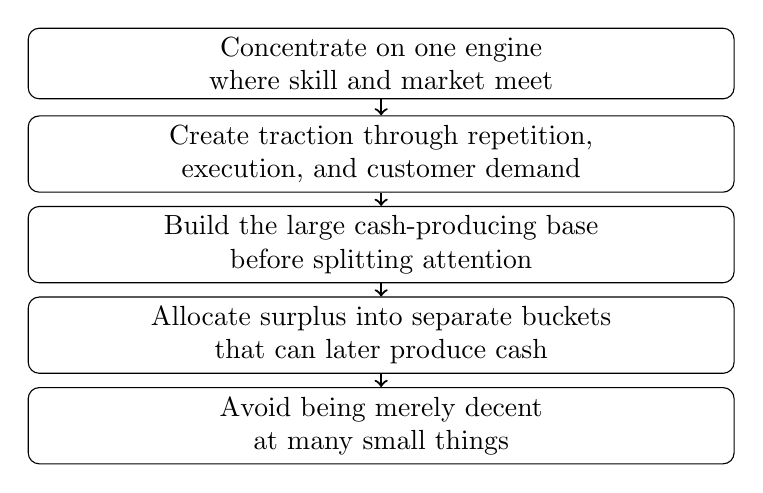
\begin{tikzpicture}[
  box/.style={draw, rounded corners, align=center, text width=0.72\linewidth, minimum height=0.72cm},
  arrow/.style={->, thick}
]
\node[box] (focus) at (0,0) {Concentrate on one engine\\where skill and market meet};
\node[box] (traction) at (0,-1.15) {Create traction through repetition,\\execution, and customer demand};
\node[box] (pile) at (0,-2.30) {Build the large cash-producing base\\before splitting attention};
\node[box] (allocate) at (0,-3.45) {Allocate surplus into separate buckets\\that can later produce cash};
\node[box] (avoid) at (0,-4.60) {Avoid being merely decent\\at many small things};
\draw[arrow] (focus) -- (traction);
\draw[arrow] (traction) -- (pile);
\draw[arrow] (pile) -- (allocate);
\draw[arrow] (allocate) -- (avoid);
\end{tikzpicture}
\caption{The concentration-before-diversification sequence, reconstructed from Mitt's answer.}
\end{figure}

The corresponding symbolic sequence is
\begin{align}
\text{skill concentration} &\longrightarrow \text{market traction},\\
\text{market traction} &\longrightarrow \text{large cash-producing base},\\
\text{large base} &\longrightarrow \{A_1,A_2,\ldots,A_n\},
\end{align}
where \(A_1,A_2,\ldots,A_n\) denote later allocations. The order is the lesson. Diversification is not the source of the first serious wealth in this account; it is what may happen after concentrated competence has produced something worth allocating.

\section{Attention As Distribution}

The interviewer then pivots to content. Mitt has a social media audience, but he does not describe the audience as a trophy. He describes it as a source of credibility, recruiting, and unexpected opportunity. The numbers he gives are
\begin{equation}
F_{\text{TikTok}}\approx 145{,}000,\qquad
F_{\text{Instagram}}\approx 25{,}000.
\end{equation}
The more important number comes from hiring. In a company-wide meeting, he says that roughly thirty to forty percent of a new-start group reported that they had followed him first and then found the job.

\begin{equation}
P(\text{new starter followed Grant first})
\approx 0.30\text{--}0.40.
\end{equation}

So the mechanism is not simply ``have followers.'' It is
\begin{align}
\text{free information} &\longrightarrow \text{personal brand},\\
\text{personal brand} &\longrightarrow \text{credibility},\\
\text{credibility} &\longrightarrow \text{recruiting and opportunities}.
\end{align}
He also says the same visibility helped produce appearances on Fox Business and other opportunities that might not have arrived even if the company had been larger but invisible.

The chapter should preserve this pivot. Social media is not a separate lifestyle topic here. It is a distribution system for trust. In a business that needs talent, reputation, and reach, attention can become part of the operating machinery.

\section{Risk, Sales, And Repeatable Skill}

The risk section begins with a strong claim and then immediately qualifies it. Risk-taking matters, but there are times to be risk-on and times to be risk-off. One must prepare for a rainy day. The useful risk is not recklessness; it is a wager on a skill that has become repeatable.

Mitt's Ferrari line gives the time preference: he would rather use the fruits of success while young, with family and responsibilities still in front of him, than defer all reward until seventy-five. The Sahara Desert line gives the portability claim: if his brain and operating ability still worked, he believes he could rebuild faster because he now knows the process.

A compact update rule for this part of the interview is
\begin{equation}
S_{t+1}=S_t+\Delta S(\text{repetition},\text{feedback},\text{rejection},\text{adaptation}),
\end{equation}
where \(S_t\) denotes practical operating skill at time \(t\). This is a reconstruction of the argument, not a stated law. It prepares us for the sales answer that follows.

\paragraph{Worked example.}
Suppose a young salesperson begins with skill \(S_0\). Each difficult selling repetition can add a small positive increment \(a\), provided that the person receives feedback and returns to the next interaction with the same standard of delivery. The simplest model is
\begin{equation}
S_n=S_0+na.
\end{equation}
But sales is not just repetition. Rejection can damage the next attempt if emotional recovery fails. Let \(\ell\) denote the performance loss from carrying the last rejection into the next conversation. Then the effective progression is
\begin{equation}
S_n=S_0+n(a-\ell).
\end{equation}
The sales lesson is to keep \(a-\ell>0\). That is why Mitt emphasizes being told no, being cursed at, being screamed at, making thousands of cold calls, knocking on doors, and still delivering the message correctly.

This makes the order of the interview important. The claim ``bet on yourself'' comes before the sales story, but the sales story explains why the bet is not merely a mood. At eighteen or nineteen, Mitt says, he was selling DirecTV in Walmart to people who did not want to talk about DirecTV while buying groceries or coming home tired from work. The value of that experience was not the product itself. It was the repeated contact with resistance, mood, background, age, and timing.

\section{Scaling Means People Doing Fundamentals}

The scaling question begins with a concrete marker. Mitt Group was closing solar deals in seventeen states:
\begin{equation}
N_{\text{states}}=17.
\end{equation}
The interviewer then asks what takes a business from six or seven figures toward eight. Mitt answers with a definition: scaling is doing the little things right at scale.

\begin{definition}
In this chapter, \emph{scale} means repeated execution of correct fundamentals by many capable people, without the founder personally supervising every action.
\end{definition}

\subsection{Question \& Answer}

\paragraph{Question.}
Why are a CRM system, a new technology, or one smart hire not enough to scale a company?

\paragraph{Answer.}
Mitt grants that tools can help, but he assigns them a limited role. They may improve performance by ten or twenty percent, but they do not by themselves double, triple, or quadruple revenue:
\begin{equation}
\Delta R_{\text{tools}}\approx 10\%\text{--}20\%,
\qquad
\Delta R_{\text{tools}}\not\approx 2R,3R,4R.
\end{equation}
The larger multiplier comes from people: many operators who know what they are doing in particular areas and can execute without the founder overshadowing them.

\begin{figure}
\centering
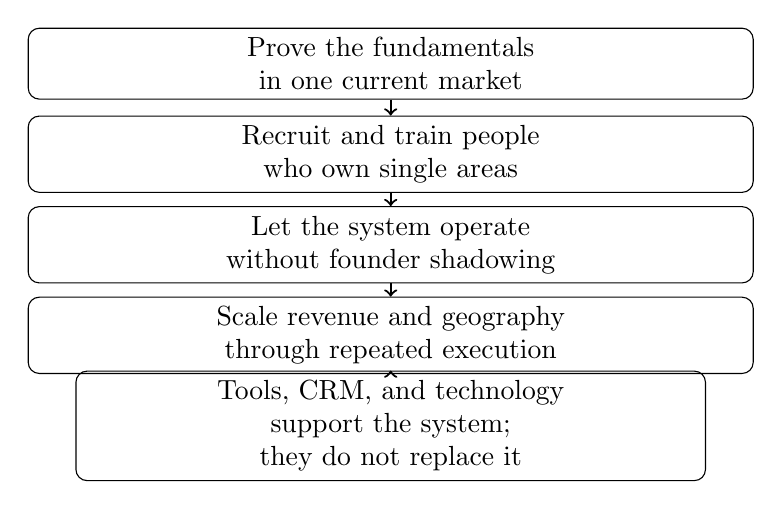
\begin{tikzpicture}[
  box/.style={draw, rounded corners, align=center, text width=0.74\linewidth, minimum height=0.70cm},
  side/.style={draw, rounded corners, align=center, text width=0.64\linewidth, minimum height=0.62cm},
  arrow/.style={->, thick}
]
\node[box] (local) at (0,0) {Prove the fundamentals\\in one current market};
\node[box] (people) at (0,-1.15) {Recruit and train people\\who own single areas};
\node[box] (delegate) at (0,-2.30) {Let the system operate\\without founder shadowing};
\node[box] (scale) at (0,-3.45) {Scale revenue and geography\\through repeated execution};
\node[side] (tools) at (0,-4.60) {Tools, CRM, and technology\\support the system;\\they do not replace it};
\draw[arrow] (local) -- (people);
\draw[arrow] (people) -- (delegate);
\draw[arrow] (delegate) -- (scale);
\draw[arrow] (scale) -- (tools);
\end{tikzpicture}
\caption{Scaling as fundamentals repeated through people, with tools in a supporting role.}
\end{figure}

This also explains the warning against premature expansion. Before we ask whether to move to another city, another state, or another country, we have to ask whether the current location is actually being conquered. Scale is not escape from fundamentals. It is fundamentals under multiplication.

\section{Energy, Industry Choice, And Team Filters}

The burnout section turns the same operating logic inward. Mitt says burnout happens when we fail to control energy and emotions. A day begins with finite energy. Communication, interaction, and decision each draw some of it down. Emotional leakage draws it down faster.

A cautious reconstruction is
\begin{equation}
E_{\text{remaining}}
=
E_{\text{day}}
-\sum_{i=1}^{n} c_i
-L_{\text{emotion}},
\end{equation}
where \(c_i\) is the energy cost of the \(i\)-th communication, interaction, decision, or appointment, and \(L_{\text{emotion}}\) is the additional loss from anger, frustration, or carryover. Mitt's example is an appointment that goes badly: if we spend energy being upset, that waste affects the next appointment.

The practical update rule is
\begin{equation}
\text{disciplined no}
\longrightarrow
\text{less wasted energy}
\longrightarrow
\text{better next action}.
\end{equation}
This is why his answer is not simply ``work less.'' It is: protect the energy that makes the next commercial action possible.

The next question asks why solar. Mitt places the choice in the years around 2014 to 2016, when he was looking for industries likely to be larger in twenty years than they were then. He names technology, artificial intelligence, robotics, renewable energy, and crypto. He does not claim that he already knew everything about those fields. The method was to identify expanding arenas, get a foot in the door, learn, and build where the crowd of conventional peers was not already going.

The closing hiring answer gives the human filter. Talent is useful, but it is not enough. School is not enough. A referral is not enough. The non-negotiables are coachability, humility, and persistence. He adds one more severe criterion: people with easy fallback plans often do not have the same necessity. The person who has to make it, in his account, keeps finding a way.

\begin{table}
\centering
\begin{tabular}{p{0.30\linewidth}p{0.58\linewidth}}
Filter & Operating meaning \\
Coachable & Can absorb the company's method rather than arriving only with prior habits \\
Humble & Can be corrected without turning correction into identity threat \\
Persistent & Continues through rejection, difficulty, repetition, and slow feedback \\
No easy fallback & Has enough necessity to keep moving when the work becomes uncomfortable \\
\end{tabular}
\caption{Mitt's hiring filters, stated as operating traits rather than credentials.}
\end{table}

\section{Summary}

The interview unfolds as a sequence of commercial tests. First, the market chooses, so age becomes secondary to trust, offer, and execution. Second, the base rates of business ownership are unattractive enough that entrepreneurship needs more than romance. Third, Mitt's own trigger was necessity under prepared conditions. Fourth, the first serious wealth engine was concentration, not early diversification. Fifth, attention mattered because it became credibility, recruiting, and opportunity flow. Sixth, risk became more rational after sales experience made skill repeatable. Seventh, scale meant people executing fundamentals without founder dependence. Finally, energy control, industry choice, and hiring all returned to the same practical discipline: protect the resource, choose expanding arenas, and find people whose traits survive pressure.